\subsection{Schutzmechanismen}

Im Kapitel Schutzmechanismen befassen wir uns mit dem Thema, wie man unsere anfällige trainierten Modelle aus Kapitel \ref{chap:modelltraining} fine tunen bzw. Schutzmechanismen anwenden, um das Modell robuster gegenüber unsere adversarial Training machen. 

\subsubsection{Data Augmentation}



\subsubsection{Input Ensembles}


\subsubsection{Adversarial Training}


\todo{Adversarial; Training beschreiben die wir verwenden, um unsere Modelle stabiler zu machen}




\subsubsection{Übersicht Modell Finetuning}
In der Abbildung \ref{fig:Evaluierungspipeline} ist der Iterationsschritt der Pipeline zu sehen. Die Pipeline wird dabei x-mal durchlaufen, was bedeutet, dass die Robustifizierung ebenfalls x-mal für das Modell und Datensatz durchgeführt wird.

\begin{figure}[H]
    \centering
    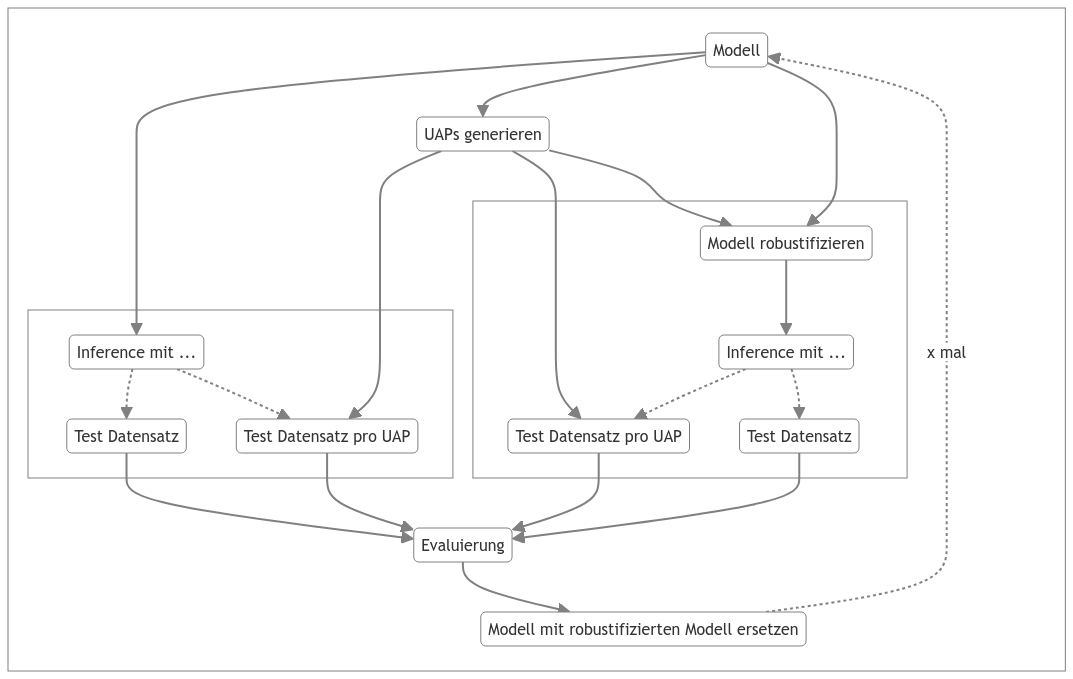
\includegraphics[width=\linewidth]{01-images/04-methodik/pipeline-robustifizierung.png}
    \caption{Übersicht der Evaluierungspipeline}
    \label{fig:Evaluierungspipeline}
\end{figure}

\begin{itemize}
    \item \textbf{Modell}: Startpunkt der Pipeline, unser trainiertes Modell auf unserem Datensatz.
    \item \textbf{UAPs generieren}: \acrshort{uap} werden generiert, um das Modell robuster zu machen.
    \item \textbf{Modell robustifizieren}: Adversarial Training wird angewendet, um das Modell zu robustifizieren. Siehe Kapitel \ref{chap:adversarial training}.
    \item \textbf{Inference mit...}: Erfolgt über zwei parallele Wege:
        \begin{itemize}
            \item Einer führt zur Inferenz mit dem ursprünglichen Modell, jeweils für den Testdatensatz mit und ohne \acrshort{uap}.
            \item Der andere Weg führt zur Inferenz mit dem robustifizierten Modell, ebenfalls für Testdatensatz mit und ohne \acrshort{uap}.
        \end{itemize}
    \item \textbf{Evaluierung}: Im Evaluierungsschritt werden vier Pakete durch die Inferenz erzeugt und miteinander verglichen.
\end{itemize}

